\documentclass[12pt,letterpaper]{article}

% --- Paquetes Básicos y de Idioma ---
\usepackage[utf8]{inputenc}
\usepackage[spanish,es-tabla]{babel}
\usepackage{geometry}
\geometry{top=2cm, bottom=2cm, left=3cm, right=3cm}

% --- Paquetes de Formato Gráfico y Tablas ---
\usepackage{graphicx}
\usepackage{booktabs}
\usepackage{titlesec}
\usepackage{fancyhdr}
\usepackage{hyperref}

% --- Paquete para Código Fuente (C/CMake) ---
\usepackage{listings}
\usepackage{xcolor}

\definecolor{mGreen}{rgb}{0,0.6,0}
\definecolor{mGray}{rgb}{0.5,0.5,0.5}
\definecolor{mPurple}{rgb}{0.58,0,0.82}
\definecolor{backgroundColour}{rgb}{0.95,0.95,0.92}

\lstset{
    backgroundcolor=\color{backgroundColour},   
    commentstyle=\color{mGreen},
    keywordstyle=\color{magenta},
    numberstyle=\tiny\color{mGray},
    stringstyle=\color{mPurple},
    basicstyle=\ttfamily\footnotesize,
    breakatwhitespace=false,         
    breaklines=true,                 
    captionpos=b,                    
    keepspaces=true,                 
    numbers=left,                    
    numbersep=5pt,                  
    showspaces=false,                
    showstringspaces=false,
    showtabs=false,                  
    tabsize=2,
    language=C
}

% --- Configuración de Encabezado y Pie de Página ---
\pagestyle{fancy}
\fancyhf{}
\lhead{Diseño de IoT y Sistemas Embebidos}
\rhead{Laboratorio 3: FreeRTOS}
\cfoot{\thepage}

% --- Datos del Documento ---
\title{
    \vspace{-1cm}
    
\includegraphics[width=0.3\textwidth]{uculogo.png} 
    \\ 
    % Reemplazar por tu imagen de logo si tienes
    \vspace{1cm}
    \textbf{Informe de Laboratorio 3: FreeRTOS}\\
    \large Multitasking y Mecanismos de Sincronización
}
\author{
    \textbf{Integrantes:}\\
    Santiago Blanco \\
    Felipe Paladino \\
    Piero Saucedo
}
\date{\today}

\begin{document}

\maketitle
\thispagestyle{empty}
\clearpage

\tableofcontents
\clearpage

% --- SECCIÓN 1: INTRODUCCIÓN ---
\section{Objetivos}
El objetivo de este laboratorio es desarrollar e implementar una arquitectura de software multitarea utilizando el sistema operativo en tiempo real \textbf{FreeRTOS} sobre el framework \textbf{ESP-IDF}. Se tiene por propósito tratar y resolver problemas de concurrencia, comunicación entre tareas y protección de recursos compartidos mediante la aplicación práctica de:
\begin{itemize}
    \item Creación, asignación de prioridades y control del ciclo de vida de las Tareas (\textit{Tasks}).
    \item Intercambio de mensajes mediante Colas (\textit{Queues}).
    \item Protección de variables críticas mediante Semáforos Mutex.
    \item Temporización diferida utilizando \textit{Software Timers} y gestión segura de memoria dinámica.
\end{itemize}

% --- SECCIÓN 2: ARQUITECTURA ---
\section{Arquitectura del Sistema}
El sistema se diseñó de forma modular respetando la estructura de componentes exigida. La arquitectura está compuesta por tres tareas principales que interactúan de manera concurrente de la siguiente forma:

\subsection{Descripción de las Tareas}
\begin{table}[h!]
    \centering
    \caption{Configuración y Prioridades de las Tareas del Sistema.}
    \begin{tabular}{llll}
        \toprule
        \textbf{Tarea} & \textbf{Componente} & \textbf{Prioridad} & \textbf{Función Principal} \\
        \midrule
        \texttt{TASK\_A} & \texttt{task\_a} & Baja (\texttt{tskIDLE\_PRIORITY+1}) & Parpadeo del LED RGB (500ms) \\
        \texttt{TASK\_B} & \texttt{task\_b} & Alta (Máxima del sistema) & Recepción y parseo de comandos UART \\
        \texttt{TASK\_C} & \texttt{task\_c} & Media & Desencolado y gestión de timers \\
        \bottomrule
    \end{tabular}
\end{table}

\subsection{Estructuras de Datos Compartidas}
De acuerdo al archivo \texttt{shared\_types.h}, se definieron las estructuras globales para el manejo de colores y comandos:

\begin{lstlisting}
typedef struct {
    uint8_t r;
    uint8_t g;
    uint8_t b;
} rgb_color_t;

typedef struct {
    rgb_color_t color;
    uint32_t delay_s;
} led_command_t;

typedef struct {
  SemaphoreHandle_t color_mutex;
  rgb_color_t *current_color; 
  led_strip_t *led_strip;
} task_a_params_t;

typedef struct {
  QueueHandle_t command_queue;
} task_b_params_t;

typedef struct {
  QueueHandle_t command_queue;
  SemaphoreHandle_t color_mutex;
  rgb_color_t *current_color;
} task_c_params_t;


\end{lstlisting}

% --- SECCIÓN 3: IMPLEMENTACIÓN ---
\section{Implementación y Sincronización}

\subsection{TASK A: Control de Parpadeo y Mutex}

La principal y única función asignada a la \textit{Task A} tiene por objeto efectuar el parpadeo del LED con un \textit{delay} de 500ms. Dado que dicho LED es un recurso que será compartido por las demás tareas, es preciso protegerlo para evitar condiciones de carrera\footnote{Una condición de carrera existe cuando el acceso a recursos compartidos no es controlado, resultando posiblemente en corrupción de datos. (Silberschatz et al., 2018)}. La función tiene por firma \texttt{void blink\_led\_task(void *pvParameters)}, como especifica la API de FreeRTOS.

La lectura de la variable global \texttt{led\_strip} es protegida por \texttt{color\_mutex}, de tipo \texttt{SemaphoreHandle\_t}. Al inicio de la función se solicita tomar el control del mutex, esperando un máximo de 500ms antes de que se considere por fracasada la solicitud como se muestra a continuación.

\begin{lstlisting}
while (1) {
    if (xSemaphoreTake(params->color_mutex, pdMS_TO_TICKS(500)) == pdTRUE) {
    
    ...

      xSemaphoreGive(params->color_mutex);
    }
    vTaskDelay(pdMS_TO_TICKS(100));
  }
}
\end{lstlisting}

Esto asegura que dos tareas que requieran acceder al recurso no choquen y fallezcan en el intento, evitando una condición de carrera.

Finalmente, la tarea es creada en el punto de entrada del proyecto con la prioridad indicada de la siguiente forma, como indica la API de FreeRTOS:
\begin{lstlisting}
xTaskCreate
    (blink_led_task,              
     "TASK_A",
     CONFIG_ESP32_PTHREAD_TASK_STACK_SIZE_DEFAULT,
     &task_a_params,
     tskIDLE_PRIORITY + 1, // priridad baja
     &task_a_handler
     );
\end{lstlisting}

\subsection{TASK B: Protocolo UART y Encolado}

La \textit{Task B} es la tarea de mayor prioridad del sistema y tiene como objetivo recibir comandos desde la consola UART. Para ello, se utilizó el driver UART provisto por ESP-IDF configurado a 115200 baudios.

El protocolo implementado utiliza un formato de texto simple:

\begin{center}
\texttt{<COLOR> <SEGUNDOS>\textbackslash n}
\end{center}

Por ejemplo:

\begin{center}
\texttt{ROJO 5}
\end{center}

La tarea permanece bloqueada esperando bytes desde la UART. Una vez recibida una línea completa, se realiza el parseo del mensaje utilizando \texttt{sscanf()}, verificando tanto el formato como la validez del color ingresado.

Si el comando es válido, se construye una estructura de tipo \texttt{led\_command\_t} y se envía a la cola compartida mediante \texttt{xQueueSend()}. En caso de error de formato o color desconocido, se registra un mensaje mediante \texttt{ESP\_LOGW()}.

Luego de encolar exitosamente el comando, la tarea responde por UART con un mensaje de confirmación para facilitar la depuración y trazabilidad del sistema.
\\

Por ejemplo:

\begin{center}
\texttt{OK rojo en 5}
\end{center}

\begin{lstlisting}
if (xQueueSend(queue, &cmd, pdMS_TO_TICKS(100)) != pdTRUE) {
    ESP_LOGW(TAG, "queue full");
    continue;
}

snprintf(ack, sizeof(ack), "OK: %s en %u\n", color_str, delay_s);

uart_write_bytes(UART_NUM_0, ack, strlen(ack));
\end{lstlisting}

\newpage

\subsection{TASK C: Gestión Dinámica de Software Timers}

La \textit{Task C} tiene como responsabilidad recibir comandos desde la cola compartida y programar la aplicación diferida del color correspondiente mediante \textit{Software Timers} de FreeRTOS. A diferencia de \textit{TASK\_A}, esta tarea no interactúa directamente con el LED físico, sino que modifica la variable compartida \texttt{current\_color}. Posteriormente, \textit{TASK\_A} lee dicha variable y realiza el parpadeo del LED con el color actualizado.

La tarea recibe como parámetro una estructura de tipo \texttt{task\_c\_params\_t}, que contiene tres elementos esenciales: la cola de comandos, el mutex que protege el color actual y un puntero a la variable compartida \texttt{current\_color}. Al iniciar, la tarea valida que los parámetros recibidos no sean nulos y luego guarda el mutex y el puntero al color actual en variables \texttt{static} internas al archivo \texttt{task\_c.c}.

\begin{lstlisting}
static SemaphoreHandle_t s_color_mutex = NULL;
static color_t *s_current_color = NULL;
\end{lstlisting}

Estas variables son necesarias porque el \textit{callback} del timer no recibe directamente la estructura de parámetros de \textit{TASK\_C}. El callback solamente recibe un \texttt{TimerHandle\_t}; por tanto, para poder acceder al mutex y a la variable compartida, se conservan referencias internas dentro del archivo.

\subsubsection{Recepción de comandos desde la cola}

El núcleo de \textit{TASK\_C} se encuentra en el uso de \texttt{xQueueReceive()}. Esta función permite que la tarea permanezca bloqueada hasta que exista un comando disponible en la cola.

\begin{lstlisting}
led_command_t command;

while (1) {
    if (xQueueReceive(params->command_queue,
                      &command,
                      portMAX_DELAY) == pdTRUE) {
        ...
    }
}
\end{lstlisting}

El tercer parámetro, \texttt{portMAX\_DELAY}, indica que la tarea debe esperar indefinidamente hasta recibir un elemento. De esta forma, \textit{TASK\_C} no consume CPU innecesariamente mientras no existan comandos pendientes. Cuando \textit{TASK\_B} recibe un comando válido por UART, construye una estructura \texttt{led\_command\_t} y la inserta en la cola mediante \texttt{xQueueSend()}. En ese momento, \textit{TASK\_C} se desbloquea y copia el comando recibido en la variable local \texttt{command}.

Por ejemplo, ante el comando UART:

\begin{center}
\texttt{azul 2}
\end{center}

\textit{TASK\_B} interpreta el texto \texttt{azul} como el color \texttt{\{0, 0, 255\}} y el valor \texttt{2} como un retardo de dos segundos. Luego encola una estructura equivalente a:

\begin{lstlisting}
led_command_t cmd;
cmd.color = (color_t){0, 0, 255};
cmd.delay_s = 2;
\end{lstlisting}

Cuando \textit{TASK\_C} recibe ese comando, se obtiene un registro de trazabilidad similar al siguiente:

\begin{lstlisting}
TASK_C: Comando recibido R=0 G=0 B=255 delay=2 s
\end{lstlisting}

\subsubsection{Reserva de memoria y creación del timer}

Una vez recibido el comando, \textit{TASK\_C} reserva memoria dinámica para almacenar una copia del color asociado al comando:

\begin{lstlisting}
color_t *timer_color = pvPortMalloc(sizeof(color_t));

if (timer_color == NULL) {
    ESP_LOGE(BALL, "No se pudo reservar memoria para el color.");
    continue;
}

*timer_color = command.color;
\end{lstlisting}

Esta reserva es necesaria porque la variable \texttt{command} es local a la tarea y puede ser sobrescrita en la siguiente iteración del ciclo. Cada timer debe conservar su propia copia independiente del color a aplicar. Por este motivo, no se pasa directamente la dirección de \texttt{command.color}, sino que se crea una copia dinámica mediante \texttt{pvPortMalloc()}.

Luego se convierte el retardo recibido en segundos a ticks de FreeRTOS:

\begin{lstlisting}
TickType_t timer_period =
    pdMS_TO_TICKS(command.delay_s * 1000);
\end{lstlisting}

FreeRTOS no trabaja internamente con segundos, sino con ticks. Por tanto, el valor \texttt{delay\_s} se multiplica por 1000 para obtener milisegundos, y luego se convierte a ticks mediante \texttt{pdMS\_TO\_TICKS()}.

Posteriormente, se crea un timer de tipo \textit{one-shot}:

\begin{lstlisting}
TimerHandle_t timer = xTimerCreate(
    "color_timer",
    timer_period,
    pdFALSE,
    timer_color,
    color_timer_callback
);
\end{lstlisting}

El parámetro \texttt{pdFALSE} indica que el timer se ejecutará una sola vez. El cuarto parámetro, \texttt{timer\_color}, queda asociado al timer como su \texttt{pvTimerID}. Esto permite que, cuando el timer venza, el callback pueda recuperar el color que debe aplicarse.

Finalmente, el timer se inicia con \texttt{xTimerStart()}:

\begin{lstlisting}
if (xTimerStart(timer, 0) != pdPASS) {
    ESP_LOGE(BALL, "Fue imposible iniciar el timer.");
    xTimerDelete(timer, 0);
    vPortFree(timer_color);
    continue;
}
\end{lstlisting}

Si el timer no pudiera iniciarse, se elimina el timer creado y se libera la memoria previamente reservada para evitar fugas de memoria.

\subsubsection{Callback del timer}

El \textit{callback} es una función que FreeRTOS ejecuta automáticamente cuando vence el timer. En este caso, la función asociada es \texttt{color\_timer\_callback()}.

\begin{lstlisting}
static void color_timer_callback(TimerHandle_t xTimer)
{
    color_t *new_color =
        (color_t *)pvTimerGetTimerID(xTimer);

    ...
}
\end{lstlisting}

La función \texttt{pvTimerGetTimerID()} permite recuperar el puntero que fue asociado al timer durante su creación. En este proyecto, dicho puntero corresponde al color que debe ser aplicado.

El callback verifica primero que el puntero recibido no sea nulo. Luego toma el mutex antes de modificar la variable compartida \texttt{current\_color}:

\begin{lstlisting}
if (xSemaphoreTake(s_color_mutex, portMAX_DELAY) == pdTRUE) {
    s_current_color->r = new_color->r;
    s_current_color->g = new_color->g;
    s_current_color->b = new_color->b;

    xSemaphoreGive(s_color_mutex);

    ESP_LOGI(BALL, "Color aplicado: R=%d G=%d B=%d",
             new_color->r,
             new_color->g,
             new_color->b);
}
\end{lstlisting}

El mutex es necesario porque \textit{TASK\_A} también accede a \texttt{current\_color} para leer el color con el cual debe parpadear el LED. De esta forma, se evita que una tarea lea la variable mientras otra la está modificando.

Luego de aplicar el color, el callback libera la memoria dinámica reservada para el color y elimina el timer:

\begin{lstlisting}
vPortFree(new_color);
xTimerDelete(xTimer, 0);
\end{lstlisting}

Esto es importante porque cada comando recibido genera un nuevo bloque de memoria y un nuevo timer. Si estos recursos no se liberaran correctamente, el sistema podría presentar fugas de memoria o acumulación innecesaria de timers ya vencidos.

\subsubsection{Flujo completo de ejecución}

El flujo completo del sistema puede resumirse de la siguiente forma:

\begin{enumerate}
    \item El usuario escribe un comando por UART, por ejemplo \texttt{azul 2}.
    \item \textit{TASK\_B} recibe la línea de texto desde UART.
    \item \textit{TASK\_B} separa el color y el retardo usando \texttt{sscanf()}.
    \item \textit{TASK\_B} transforma el texto \texttt{azul} en el color \texttt{\{0,0,255\}}.
    \item \textit{TASK\_B} construye un \texttt{led\_command\_t}.
    \item \textit{TASK\_B} encola el comando mediante \texttt{xQueueSend()}.
    \item \textit{TASK\_C}, que estaba bloqueada en \texttt{xQueueReceive()}, recibe el comando.
    \item \textit{TASK\_C} reserva memoria dinámica para guardar una copia del color.
    \item \textit{TASK\_C} crea e inicia un timer \textit{one-shot} con el retardo indicado.
    \item Cuando vence el timer, FreeRTOS ejecuta el callback.
    \item El callback recupera el color con \texttt{pvTimerGetTimerID()}.
    \item El callback toma el mutex y actualiza \texttt{current\_color}.
    \item \textit{TASK\_A}, en su siguiente ciclo, lee \texttt{current\_color} y parpadea el LED con el nuevo color.
\end{enumerate}

En síntesis, \textit{TASK\_B} produce comandos, \textit{TASK\_C} los programa temporalmente mediante timers, y \textit{TASK\_A} refleja visualmente el estado actual del color en el LED RGB.

\newpage

% --- SECCIÓN 4: RESULTADOS ---
\section{Resultados y Pruebas}

Durante las pruebas realizadas se verificó el correcto funcionamiento del sistema multitarea implementado con FreeRTOS. A través del monitor serie de ESP-IDF fue posible observar la inicialización de las tareas, la recepción y parseo de comandos UART, el encolado de estructuras \texttt{led\_command\_t} y la posterior aplicación de colores mediante timers.

La Figura \ref{fig:monitor} muestra una ejecución típica del sistema utilizando comandos enviados por UART.

\begin{figure}[h!]
    \centering
    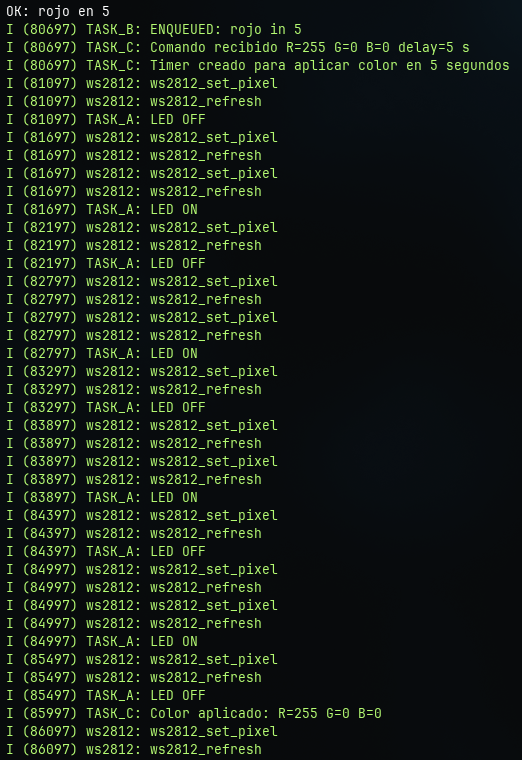
\includegraphics[width=0.55\textwidth]{results.png}
    \caption{Salida del monitor serie mostrando recepción de comandos, encolado y aplicación de colores.}
    \label{fig:monitor}
\end{figure}
\clearpage

% --- SECCIÓN 5: EXTENSIONES ---
% \section{Extensiones Implementadas (Opcional)}
% \textit{Nota: Si se implementó alguna mejora opcional (como cola con timeout, cancelación de timers pendientes, comando de estado, monitor de stack o efectos de transición), detallar su funcionamiento y diseño aquí.}

% --- SECCIÓN 6: CONCLUSIONES ---
\section{Conclusiones}
El objetivo de este laboratorio fue alcanzado con éxito, permitiendo analizar diversas cuestiones concernientes a la comunicación y sincronización de procesos usando estructuras propias del sistema operativo FreeRTOS. 

En definitiva, se evidenció claramente la necesidad del uso de herramientas como mutex para evitar condiciones de carrera, colas para intercambio de mensajes entre los procesos, y temporización en el marco de un sistema operativo de tiempo real usando timers por software. 

\newpage
\section{Bibliografía}

\begin{itemize}
    \item Tanenbaum, A. S. (2009). \textit{Sistemas Operativos Modernos} (3.ª ed.). Pearson Educación.
    \item Silberschatz, A., Galvin, P. B., \& Gagne, G. (2018). \textit{Operating System Concepts} (10th ed.). Wiley.
    \item Real Time Engineers Ltd. (s. f.). \textit{FreeRTOS Reference Manual}. Recuperado de \url{https://www.freertos.org/Documentation/}
\end{itemize}
\end{document}
